%!TeX spellcheck = pt_BR
\documentclass[brazil]{beamer}
%\usepackage[timeinterval=1,font=Helv]{tdclock}
\usetheme{Frankfurt}
\useoutertheme[subsection=false,footline=authortitle]{miniframes}
%\useoutertheme{shadow}


%\usepackage{beamerthemesplit}
%\usepackage{ragged2e}
%\usepackage{etoolbox}
\usepackage{hyphenat}
\usepackage{babel}
%\hyphenation{mate-mática recu-perar}
\usepackage[T1]{fontenc}
\usepackage{lmodern}
\usepackage[utf8x]{inputenc}
\usepackage[figurename=Imagem]{caption}
\usepackage[alf,abnt-etal-cite=2]{abntex2cite}
\usepackage{multirow}
\usepackage{tikz}
% use our .sty file for simple movie commands
\usepackage{pdfpc-commands}
%\usepackage{remreset}
%\makeatletter
%\@removefromreset{subsection}{section}
%\makeatother
%\setcounter{subsection}{1}

%\usetheme{Darmstadt}
%\setbeamerfont*{frametitle}{size=\normalsize,series=\bfseries}
%\setbeamertemplate{navigation symbols}{}
%\addtobeamertemplate{navigation symbols}{}{%
%    \usebeamerfont{footline}%
%    \usebeamercolor[fg]{footline}%
%    \hspace{1em}%
%    \insertframenumber/\inserttotalframenumber
%}
\setbeamertemplate{navigation symbols}{}
\setbeamercovered{transparent=20}
\newcommand*\oldmacro{}%
\let\oldmacro\insertshorttitle%
\renewcommand*\insertshorttitle{%
  \oldmacro\hfill%
  \insertframenumber/\inserttotalframenumber}

\setbeamertemplate{headline}
 {%
  \begin{beamercolorbox}{section in head/foot}
  \insertsectionnavigationhorizontal{\textwidth}{}{}
  \end{beamercolorbox}%
}

\AtBeginSection[]
{
  \begin{frame}
    \frametitle{Conteúdo}
    \tableofcontents[currentsection]
  \end{frame}
}


\title[Detecção de efeitos colaterais indesejáveis na Internet das coisas...]{Detecção de efeitos colaterais indesejáveis na Internet das coisas - um estudo de caso no Home Network System}
\subtitle{Apresentação de Monografia}
\author[Heron Sanches Gonçalves Pires Ferreira]{
  Heron Sanches Gonçalves Pires Ferreira
}


\institute[UFBA]{
  \\Universidade Federal da Bahia
  \\Departamento de Ciência da Computação
  \\\textbf{Orientadora:} Profa. Dra. Daniela Barreiro Claro 
  \\Contato: \email{heronsanches@dcc.ufba.br} 
}
\date{31 de outubro de 2016}


%\setbeamertemplate{headline}{}

%\setbeamertemplate{background}{\hspace{.5em}\textcolor{red}{\tiny\bfseries\tdtime}}

\begin{document}
\begin{frame}
  \maketitle

  %\initclock

\end{frame}

\begin{frame}
  \frametitle{Conteúdo}
  \tableofcontents
\end{frame}

\section{Introdução}

\begin{frame}{Introdução}
  \begin{itemize}
    \item<1 -> O avanço da tecnologia tem proporcionado um \alert{aumento gigantesco} na quantidade
      de \alert{dados armazenados}.
    \item<2 -> A rede social Facebook produz mais de \alert{25 $terabytes$/dia} \cite{Havens2012}.
    \item<3 -> Governos e corporações também produzem milhares de \alert{documentos} todos os dias,
      tais como relatórios, formulários, pesquisas de opiniões e etc.
    \item<4 -> \citeonline{Muggleton2006} ressalta que este cenário está além dos limites humanos
      para o uso e compreensão.
  \end{itemize}
\end{frame}

\begin{frame}{Introdução}
  \begin{itemize}
    \item<1 -> \citeonline{Kobayashi2008} enfatizam que instituições estão sobrecarregadas com
      o processamento desse montante de dados. 
    \item<2 -> Os dados possuem diversos tipos e formatos, sendo armazenados de forma estruturada ou
      \alert{não estruturada}.
  \end{itemize}
  \begin{examples}<3 ->
    documentos de textos, planilhas, áudios, imagens, vídeos, documentos HTML e etc.
  \end{examples}
\end{frame}

\begin{frame}{Introdução}
  \begin{itemize}
    \item<1 -> Dados estruturados já possuem mecanismos eficientes de armazenamento e recuperação.
    \item<2 -> \alert{Documentos textuais} por serem \alert{não estruturados} são recuperados
      através de Sistemas de Recuperação da Informação (SRI). 
  \end{itemize}
  \begin{examples}<2 ->
    Duckduckgo, Jus Brasil, IEEExplore, ACM, Google e etc 
  \end{examples}
\end{frame}

%\begin{frame}{Introdução}
%  As seguintes áreas vem explorando e propondo técnicas para otimizar esse processo: 
%  \begin{itemize}
%    \item Mineração de Dados (MD) 
%    \item Aprendizado de Máquina  
%    \item Recuperação da Informação (RI)
%  \end{itemize}
%\end{frame}

\begin{frame}{Introdução}
  \begin{itemize}
    \item Demanda crescente para desenvolvimento e aprimoramento de métodos que possam
      processar e \alert{extrair padrões} de \alert{dados textuais}. 
    \item A extração de padrões de documentos textuais é o principal objetivo da Mineração de Textos
      (MT).
  \end{itemize}
\end{frame}

\begin{frame}{Introdução}
  Vários desafios estão presentes no processo de extração de padrões de documentos textuais, entre
  eles destaca-se:
  \begin{itemize}
    \item<1 -> Não estruturados.
    \item<2 -> Naturalmente \alert{imprecisos} e \alert{incertos}. 
    \item<3 -> Abordam um ou mais temas. 
    \item<4 -> \alert{Alta dimensionalidade}.
    \item<5 -> Dados \alert{esparsos}.
  \end{itemize}
  \begin{examples}<5 ->
    Uma coleção de documentos pode conter 100.000 palavras, enquanto um documento pode conter apenas
    algumas centenas \cite{Aggarwal2012}.
  \end{examples}
\end{frame}

{ % all template changes are local to this group.
    \setbeamertemplate{navigation symbols}{}
    \begin{frame}[plain,label=scatered]
        \begin{tikzpicture}[remember picture,overlay]
          \node[at=(current page.center)](img) {
            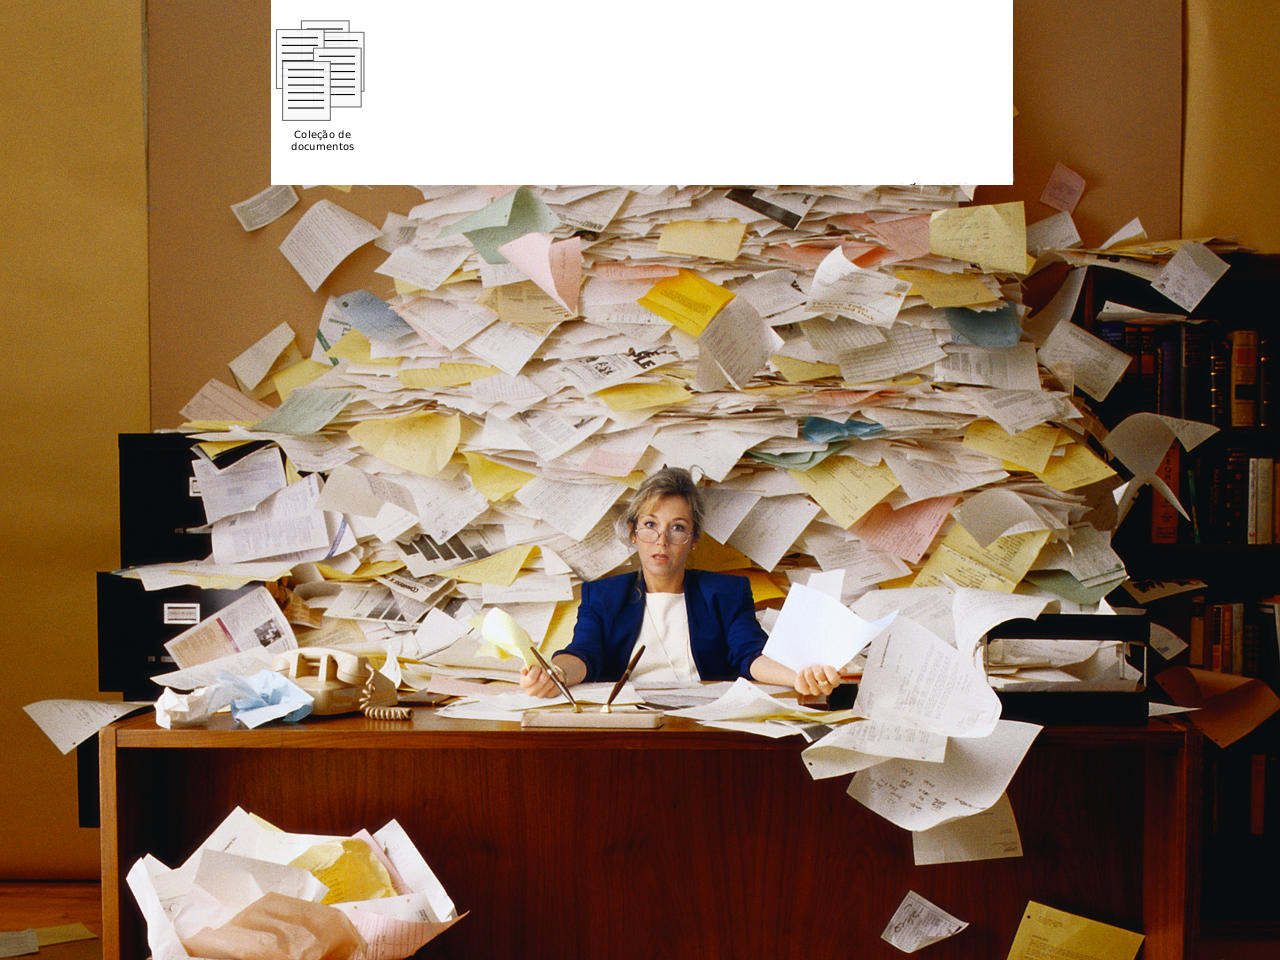
\includegraphics[width=\paperwidth]{assets/slide/scatered2.jpg}
          };
          \node[above right,text width=14cm,align=left] at (img.south west){{\color{white}Retirado
          de \url{businessblogshub.com}}};
        \end{tikzpicture}
     \end{frame}
}
{ % all template changes are local to this group.
    \setbeamertemplate{navigation symbols}{}
    \begin{frame}[plain,label=preprocessing]
        \begin{tikzpicture}[remember picture,overlay]
          \node[at=(current page.center)](img) {
            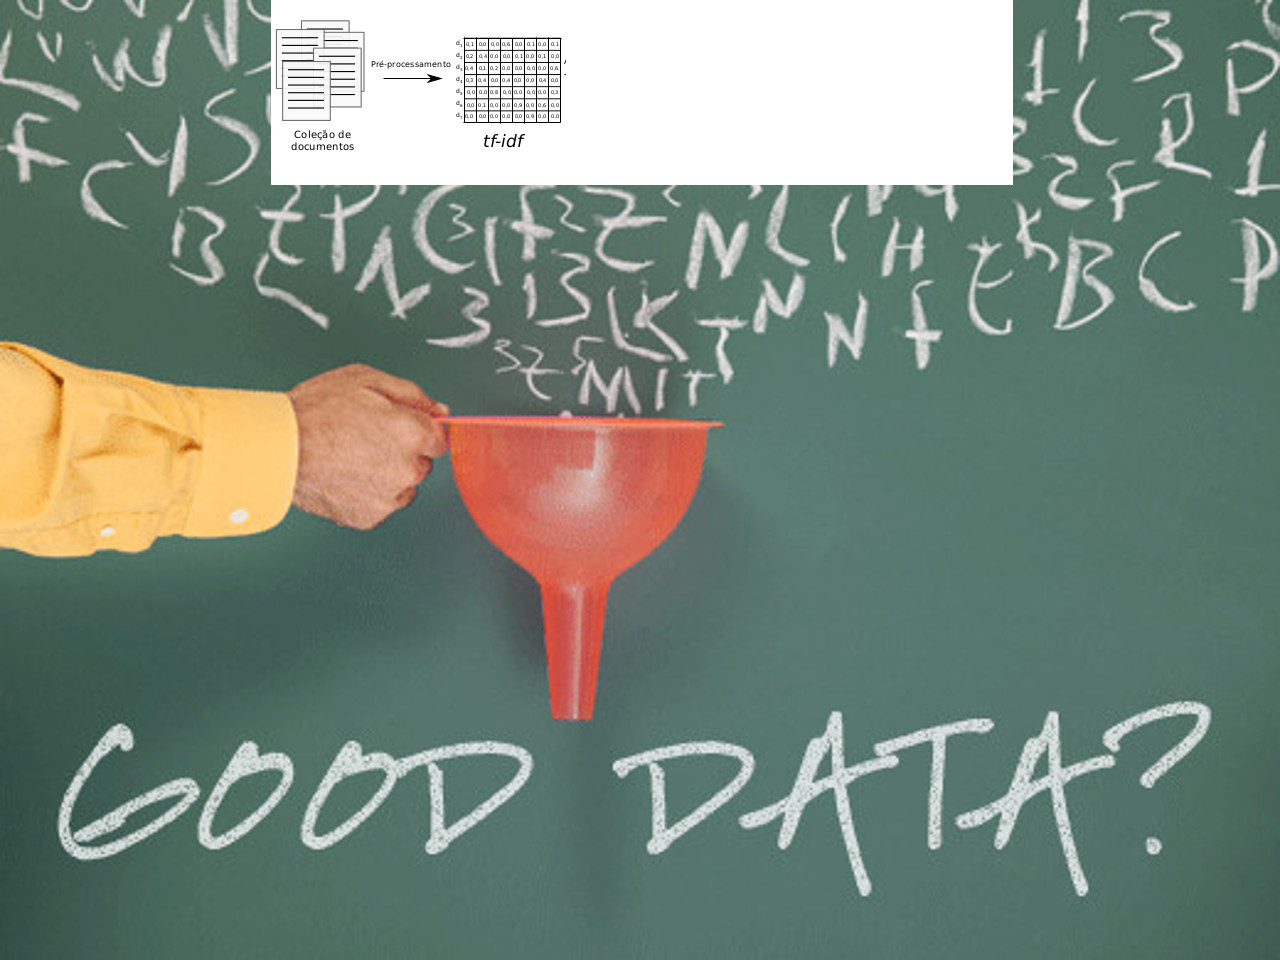
\includegraphics[width=\paperwidth]{assets/slide/processing2.jpg}
          };
          \node[above right,text width=14cm,align=left] at (img.south west){{\color{white}Retirado
          de \url{realvalidation.com}}};
        \end{tikzpicture}
     \end{frame}
}
{ % all template changes are local to this group.
    \setbeamertemplate{navigation symbols}{}
    \begin{frame}[plain,label=clustering]
        \begin{tikzpicture}[remember picture,overlay]
          \node[at=(current page.center)](img) {
            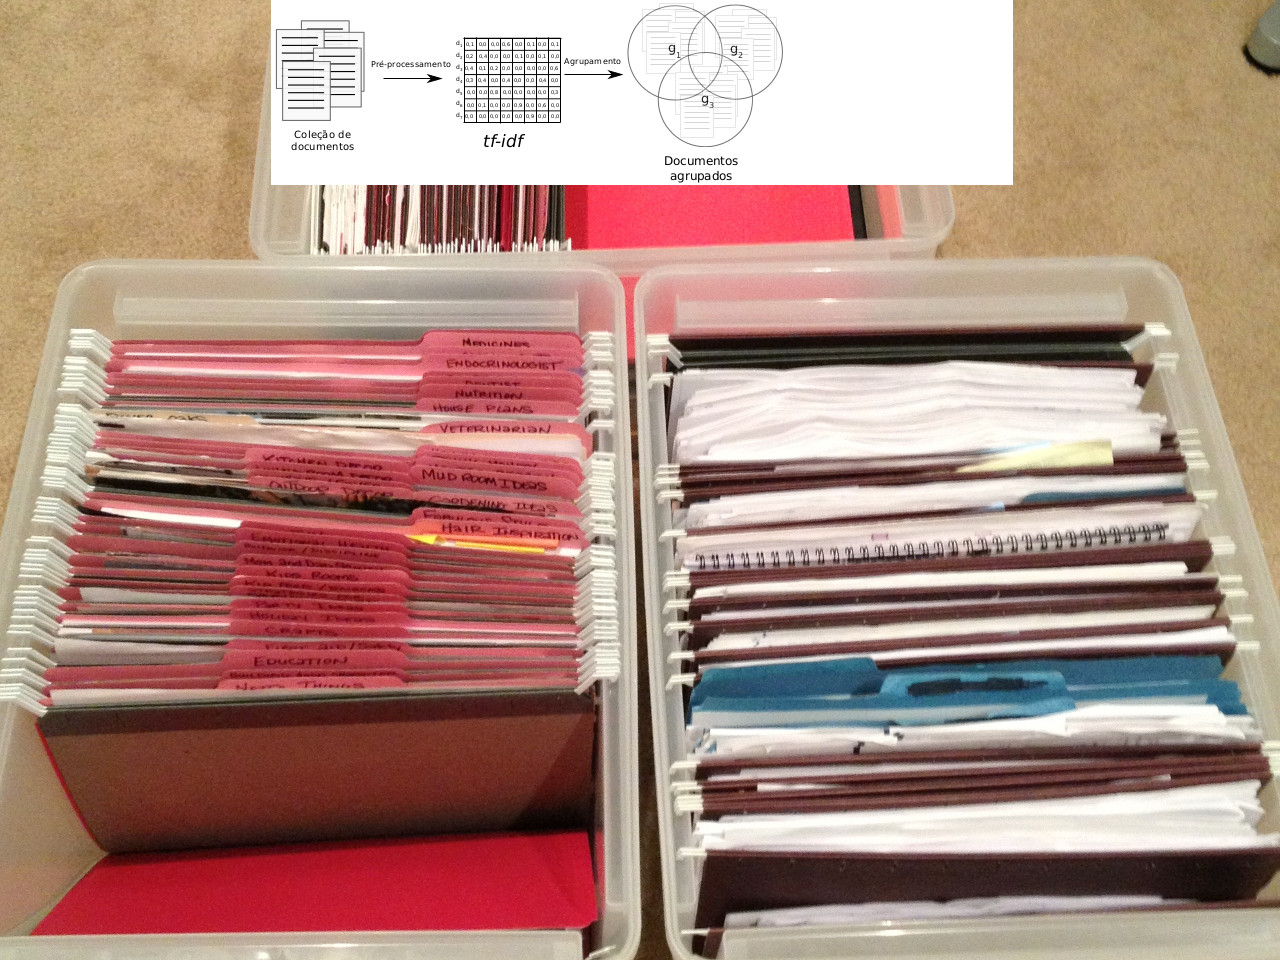
\includegraphics[width=\paperwidth]{assets/slide/box2.jpg}
          };
          \node[above right,text width=14cm,align=left] at (img.south
          west){{\color{white}Retirado de \url{fabulouslyorganizedhome.com}}};
        \end{tikzpicture}
     \end{frame}
}
{ % all template changes are local to this group.
    \setbeamertemplate{navigation symbols}{}
    \begin{frame}[plain,label=descriptors]
        \begin{tikzpicture}[remember picture,overlay]
          \node[at=(current page.center)](img) {
            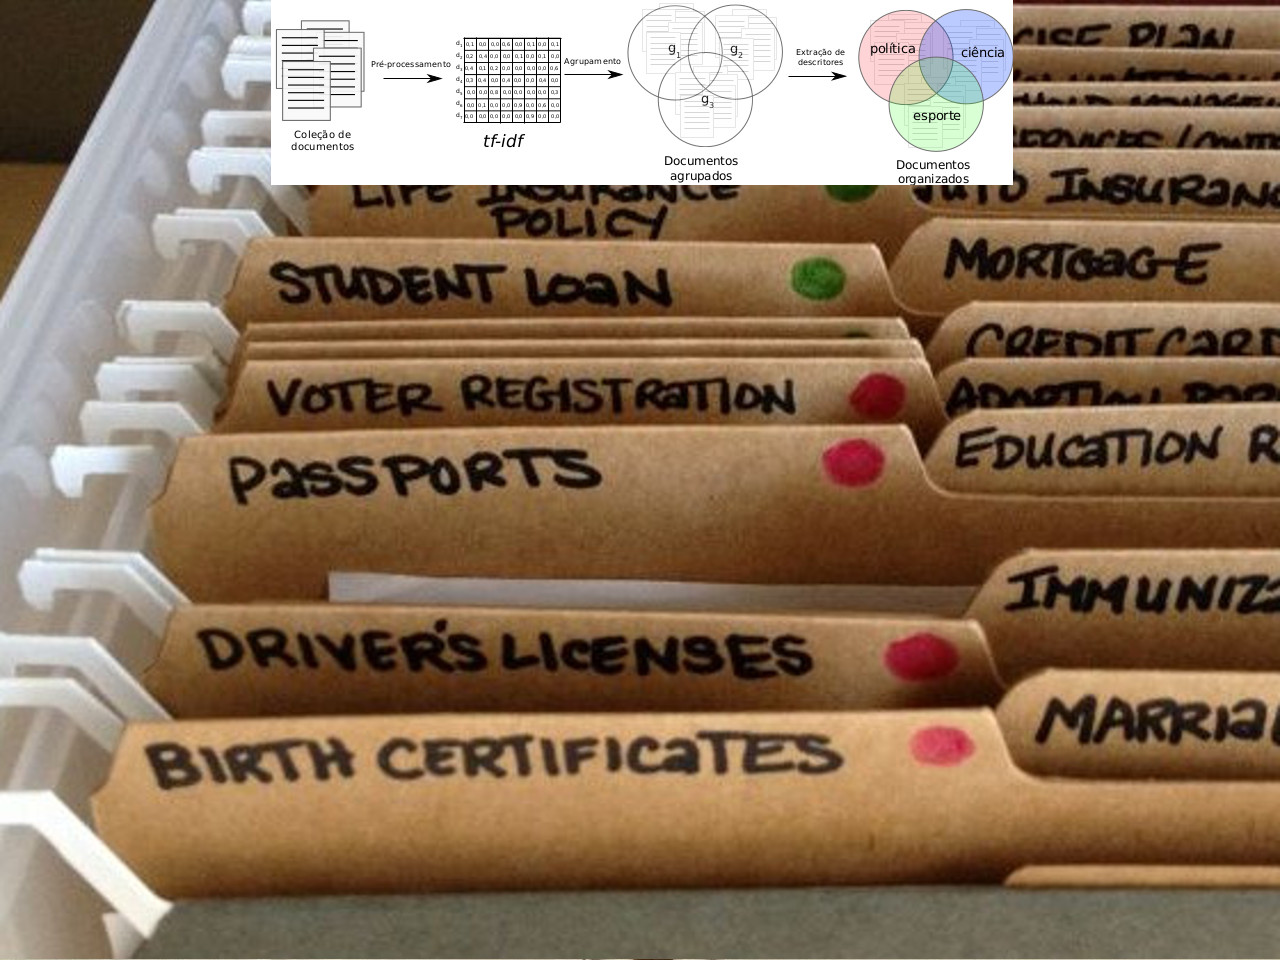
\includegraphics[width=\paperwidth]{assets/slide/organized2.jpg}
            };
            \node[above right,text width=14cm,align=left] at (img.south
            west){{\color{white}Retirado de
            \url{www.pinterest.com}}};
        \end{tikzpicture}
     \end{frame}
}
%\fullFrameImage{assets/slide/scatered.jpg}{\copyrightText{\url{https://fabulouslyorganizedhome.com/}}}
%\fullFrameImage{assets/slide/box.jpg}{}
%\fullFrameImage{assets/slide/organized.jpg}{}
%\fullFrameImage{assets/slide/scatered.jpg}{\copyrightText{Apollo 17, NASA}}

%\begin{frame}{Introdução}
%  A organização flexível de documentos se apresenta então como o processo para estruturar e
%  organizar documentos textuais considerando a incerteza e imprecisão.
%\end{frame}

\begin{frame}{Introdução}
  O agrupamento é muito importante neste processo e possui uma série de desafios:
  \begin{itemize}
    \item<1 -> Agrupar de acordo com a similaridade. 
    \item<2 -> \textbf{Grupos com significado relevante}.
    \item<3 -> Escalável para grandes coleções ({\it Big Data\/}).
    \item<4 -> Baixo custo computacional.
    \item<5 -> Estimar os parâmetros dos algoritmos.
    \item<6 -> \textbf{Considerar a imprecisão e a incerteza}.
    \item<7 -> \textbf{Reduzir a influência de \alert{documentos ruidosos}}. 
  \end{itemize} 
\end{frame}

\begin{frame}{Introdução}
  \begin{block}{Citação}
    {\it [...] não é esperado que um único método de agrupamento atenda
    todas as exigências para todos os conjuntos de dados [...] \cite{Steinbach2004}\/}.
  \end{block}
\end{frame}

\begin{frame}{Introdução}
  Existem diversos métodos de agrupamento na literatura, os quais destacam-se:
  \begin{itemize}
    \item {\it Fuzzy C-Means\/} (FCM) 
    \item {\it Possibilistic C-Means\/} (PCM) 
    \item {\it Possibilistic Fuzzy C-Means\/} (PFCM) 
  \end{itemize} 

\end{frame}

%\begin{frame}{Introdução}
%  Foi então formulada a seguinte hipótese: 
%  \begin{block}{Hipótese}
%    A utilização de uma estratégia \alert{híbrida} de agrupamento e extração de descritores, entre
%    os graus de pertinência e tipicidade providos pelo método de agrupamento PFCM, permitem o
%    aumento da robustez e resiliência contra \alert{ruídos} na \alert{organização flexível de
%    documentos}, aumentando assim a relevância dos grupos obtidos.
%  \end{block}
%
%\end{frame}
%
%\begin{frame}{Introdução}
%  Para validar a hipótese definiu-se o como objetivo desta monografia:
%
%  \begin{block}{Objetivo}
%    Conduzir uma investigação em torno dos métodos de agrupamento \textbf{FCM, PCM e PFCM}, para
%    compreender e interpretar corretamente as peculiaridades de se extrair descritores a partir de um
%    \textbf{agrupamento híbrido}.
%  \end{block}
%\end{frame}

\begin{frame}{Introdução}
  A partir das investigações conduzidas foi proposto dois métodos de extração de descritores:

  \begin{itemize}
    \item \textbf{Possibilistic Description Comes Last} (PDCL)
    \item \textbf{Mixed - Possibilistic Fuzzy Description Comes Last} (Mixed-PFDCL) (Híbrido)
  \end{itemize} 
\end{frame}

%\begin{frame}{Introdução}
%  A partir das investigações conduzidas descobriu-se que os \alert{graus de tipicidade}
%  \alert{afetam} a qualidade dos descritores dos grupos. 
%
%  Essa descoberta motivou a proposição dos métodos de extração de descritores:
%
%  \begin{itemize}
%    \item \textbf{Possibilistic Description Comes Last} (PDCL)
%    \item \textbf{Mixed - Possibilistic Fuzzy Description Comes Last} (Mixed-PFDCL) (Híbrido)
%  \end{itemize} 
%\end{frame}

\section{Fundamentação Teórica}

\subsection{Pré-processamento}

\againframe{preprocessing}
\begin{frame}{Pré-processamento}
  \begin{columns}
    \column{0.5\textwidth}
    \begin{itemize}
      \item Remoção de espaços. 
      \item Expansão de abreviações. 
      \item Remoção de {\it stopwords\/} (pronomes, artigos e etc.). 
      \item Lematização (Casa $\rightarrow$ Cas). 
      \item Estruturação dos documentos (TF-IDF). 
    \end{itemize} 

    \column{0.5\textwidth}
    \begin{table}[!htp]
      \centering
      \begin{tabular}{ |l|c|c|c|}
        \hline
        & {\bf$termo_1$} & {\bf $termo_2$} & {\bf $termo_3$} \\
        \hline
        $doc_1$ & 1 & 3 & 4 \\
        \hline
        $doc_2$ & 9 & 2 & 0 \\
        \hline
      \end{tabular}
      \caption{Exemplo matriz docs x termos}
    \end{table}
    \centering
    $\Downarrow$
    \begin{table}[!htp]
      \centering
      \begin{tabular}{ |l|c|c|c|}
        \hline
        & {\bf$termo_1$} & {\bf $termo_2$} & {\bf $termo_3$} \\
        \hline
        $doc_1$ & 0.1 & 0.6 & 1.0 \\
        \hline
        $doc_2$ & 0.9 & 0.4 & 0.0 \\
        \hline
      \end{tabular}
      \caption{Exemplo matriz tf-idf}
    \end{table}
  \end{columns}
\end{frame}

\subsection{Agrupamento (FCM,PCM,PFCM)}

\againframe{clustering}
\begin{frame}{Agrupamento}
  \begin{itemize}
    \item<1 -> Organizar objetos similares em um mesmo grupo. 
    \item<2 -> Grupos crisp x fuzzy
    \item<3 -> Coeficiente de similaridade de cosseno.
    \item<4 -> Validação do agrupamento com o método silhueta fuzzy.
  \end{itemize} 
  \visible<2 ->{
    \begin{figure}[!htp]
      \centering 
      \begin{minipage}{0.45\textwidth} 
        \centering
        \includegraphics[width=0.6\columnwidth]{assets/clusters_crisp.pdf} 
        \caption{Grupos crisp} 
      \end{minipage}\hfill 
      \begin{minipage}{0.45\textwidth} \centering
        \includegraphics[width=0.6\columnwidth]{assets/clusters_fuzzy.pdf} 
        \caption{Grupos fuzzy}
        \label{fig:cluster_fuzzy} 
      \end{minipage} 
    \end{figure}
  }
\end{frame}

\begin{frame}{Agrupamento (FCM) \cite{Bezdek1984}}
  \begin{columns}
    \column{0.5\textwidth}
    \begin{itemize}
      \item Graus de pertinência. 
      \item \alert{Restrição probabilística}.
      \item Problema com ruídos. 
    \end{itemize} 
    \begin{table}[!htp]
      \centering
      \begin{tabular}{ |l|c|c|c|}
        \hline
        & {\bf$grupo_1$} & {\bf $grupo_2$} & {\bf \alert{total}} \\
        \hline
        $doc_1$ & 0,5 & 0,5 & 1,0 \\
        \hline
        $doc_2$ & 0,5 & 0,5 & 1,0 \\
        \hline
      \end{tabular}
      \caption{Pertinências FCM}
    \end{table}

    \column{0.5\textwidth}
    \begin{figure}[!htp] \centering
      \includegraphics[width=1.0\columnwidth]{assets/fcm_problem.pdf} 
      \caption{Problema dos ruídos} 
      \label{fig:fcm_problem} 
    \end{figure}
  \end{columns}
\end{frame}

\begin{frame}{Agrupamento (PCM) \cite{Krishnapuram1993}}
  \begin{columns}
    \column{0.5\textwidth}
    \begin{itemize}
      \item Graus de tipicidade. 
      \item \alert{Remoção da restrição probabilística}.
      \item Problema dos grupos coincidentes. 
    \end{itemize} 
    \begin{table}[!htp]
      \centering
      \begin{tabular}{ |l|c|c|c|}
        \hline
        & {\bf$grupo_1$} & {\bf $grupo_2$} & {\bf \alert{total}} \\
        \hline
        $doc_1$ & 0,7 & 0,7 & 1,4 \\
        \hline
        $doc_2$ & 0,2 & 0,2 & 0,4 \\
        \hline
      \end{tabular}
      \caption{Tipicidades PCM}
    \end{table}

    \column{0.5\textwidth}
    \begin{figure}[!htp] \centering
      \includegraphics[width=1.0\columnwidth]{assets/clusters_pcm_problem.pdf} 
      \caption{Grupos coincidentes} 
      \label{fig:fcm_problem} 
    \end{figure}
  \end{columns}
\end{frame}

{ % all template changes are local to this group.
    \setbeamertemplate{navigation symbols}{}
    \begin{frame}[plain,label=fusion]
        \begin{tikzpicture}[remember picture,overlay]
          \node[at=(current page.center)](img) {
            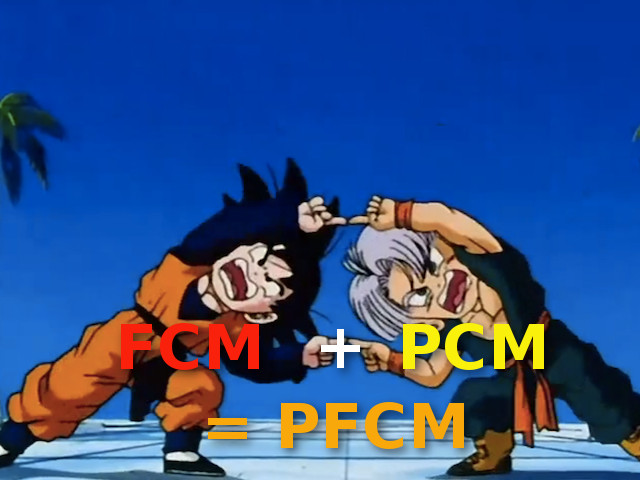
\includegraphics[width=\paperwidth]{assets/slide/fcm-and-pcm.jpg}
          };
          \node[above right,text width=14cm,align=left] at (img.south west){{\color{white}Retirado
          de \url{fanpop.com}}};
        \end{tikzpicture}
     \end{frame}
}
\begin{frame}{Agrupamento (PFCM) \cite{Pal2005}}
  \begin{columns}
    \column{0.5\textwidth}
    \begin{itemize}
      \item Pertinências e tipicidades. 
      \item Robustez. 
      \item Parâmetros de ponderação $a$ e $b$.
    \end{itemize} 

    \begin{figure}[!htp] 
      \centering 
      \includegraphics[width=1.0\columnwidth]{assets/samples_pfcm.png}
      \caption{Agrupamento de pontos.} 
      \label{fig:samples_pfcm} 
    \end{figure}

    \column{0.5\textwidth}
    \begin{table}[!htp]
      \centering
      \begin{tabular}{ |l|c|c|c|}
        \hline
        & {\bf$grupo_1$} & {\bf $grupo_2$} & {\bf total} \\
        \hline
        $doc_1$ & 0,5 & 0,5 & 1,0 \\
        \hline
        $doc_2$ & 0,5 & 0,5 & 1,0 \\
        \hline
      \end{tabular}
      \caption{Pertinências PFCM}
    \end{table}
    \begin{table}[!htp]
      \centering
      \begin{tabular}{ |l|c|c|c|}
        \hline
        & {\bf$grupo_1$} & {\bf $grupo_2$} & {\bf total} \\
        \hline
        $doc_1$ & 0,7 & 0,7 & 1,4 \\
        \hline
        $doc_2$ & 0,2 & 0,2 & 0,4 \\
        \hline
      \end{tabular}
      \caption{Tipicidades PFCM}
    \end{table}
  \end{columns}
\end{frame}

\subsection{Extração de descritores}

\againframe{descriptors}
\begin{frame}{Extração de descritores}
  \begin{itemize}
    \item<1 -> Atribuir significados aos grupos. 
    \item<2 -> Manual ou \textbf{Automatizada}. 
    \item<3 -> Abordagens de conhecimento interno e externo.
    \item<4 -> Durante o agrupamento ({\it Description Comes First\/} - DCF) 
    \item<4 -> \textbf{Após o agrupamento ({\it Description Comes Last\/} - DCL)}.
    \item<5 -> Método {\it Soft Organization - Fuzzy Description Comes Last\/} (SoftO-FDCL)
      \cite{Nogueira2013}.
  \end{itemize} 
  \begin{figure}[!htp] 
    \centering 
    \includegraphics[width=0.4\columnwidth]{assets/descriptors.pdf}
    \caption{Descritores} 
  \end{figure}
\end{frame}

%\begin{frame}{Organização Flexível de Documentos}
%  \begin{figure}[!htp] 
%    \centering 
%    \includegraphics[width=1.0\columnwidth]{assets/process.pdf}
%    \caption{Organização flexível de documentos.} 
%  \end{figure}
%  \begin{block}{Definição}<2 ->
%    A \alert{organização flexível de documentos} pode ser definida como o processo que compreende a
%    \alert{estruturação dos dados}, a adição de flexibilidade proporcionada pelo \alert{agrupamento
%    fuzzy}, a \alert{extração de descritores} dos grupos de maneira flexível e a recuperação de
%    informação através de um SRI.
%  \end{block}
%\end{frame}

\section{Trabalhos relacionados}

\begin{frame}{Trabalhos relacionados}
  \begin{itemize}
  \item<1 -> \citeonline{MarcaciniR10} propões uma abordagem incremental hierárquica para construção
    de tópicos.
  \item<2 -> \citeonline{Havens2012} e \citeonline{Kumar2015} explora otimizações para {\it Big
    Data\/}.
  \item<3 -> \citeonline{Deng2010} propõe uma maneira de estabilizar a inicialização do agrupamento.
  \item<4 -> \citeonline{Karami2015} utiliza o agrupamento ainda na fase de pré-processamento.
  \end{itemize}
\end{frame}
\begin{frame}{Trabalhos relacionados}
  \begin{itemize}
  \item<1 -> \citeonline{Jiang2013} combina os algoritmos genéticos no agrupamento para evitar os
    mínimos locais.
  \item<2 -> \citeonline{Murali2015} propõe uma medida de similaridade com informações semânticas. 
  \item<3 -> \citeonline{Nogueira2013} traz uma abordagem de extração de descritores independente do
    agrupamento.
  \end{itemize}
\end{frame}

\section{Abordagem proposta}

\begin{frame}{Coleções textuais}
  \begin{table}[!htp]
    \centering
    \begin{tabular}{ |l|c c c c c|}
      \hline
      {\bf Coleção} & {\bf docs} & {\bf termos} & {\bf classes} & {\bf \alert{\% zeros}} & {\bf
    n-gramas} \\
      \hline
      Opinosis & 51 & 842 & 3         & \alert{95,73\%} & 1-grama \\
      \hline
      20newsgroups & 2000 & 11028 & 4 & \alert{99,11\%} & 1-grama \\
      \hline
      Hitech & 600 & 6925 & 6         & \alert{97,93\%} & 1-grama \\
      \hline
      NSF & 1600 & 2806 & 16          & \alert{99,76\%} & 1-grama \\
      \hline
      WAP & 1560 & 8070 & 20          & \alert{98,51\%} & 1-grama \\
      \hline
      Reuters-21578 & 1052 & 3925 & 43 & \alert{98,55\%} & 1-grama \\
      \hline
    \end{tabular}
    \caption{Características das coleções textuais utilizadas nesta pesquisa}
    \label{table:datasets}
  \end{table}
\end{frame}

\subsection{Refinamento com PFCM}

\begin{frame}{Refinamento com PFCM}
  \begin{figure}[!htp] 
    \centering
    \includegraphics[width=1.0\columnwidth]{assets/process_pfcm.pdf} 
    \caption{Estratégia de organização flexível de documentos adotada ao se misturar abordagens fuzzy
    e possibilísticas no agrupamento} 
    \label{fig:flexibleorganization} 
  \end{figure}
\end{frame}

\begin{frame}{Refinamento com PFCM}
\begin{table}[!htp]
  \centering
  \begin{tabular}{ |l|c|c|c|c|}
    \hline
    {\bf Coleção} & {\bf \# classes} & {\bf FCM} & {\bf PCM} & {\bf PFCM} \\
    \hline
    Opinosis      & 3 &   \alert{3}   & 3 & {\color{blue}3} \\
    \hline
    20Newsgroup   & 4 &   \alert{2}   & 2 & {\color{blue}2} \\
    \hline
    Hitech        & 6 &   \alert{6}   & 5 & {\color{blue}5} \\
    \hline
    NSF           & 16 &  \alert{11}  & 2 & {\color{blue}16} \\
    \hline
    WAP           & 20 &  \alert{14}  & 5 & {\color{blue}16} \\
    \hline
    Reuters-21578 & 43 &  \alert{22}  & 11 & {\color{blue}36} \\
    \hline
  \end{tabular}
  \caption{Quantidade ótima de grupos determinada através do método da silhueta fuzzy para cada
  algoritmo de agrupamento}
  \label{table:pfcmclusters}
\end{table}
\end{frame}

\begin{frame}{Refinamento com PFCM}

  \begin{table}[!htp]
    \centering
    \begin{tabular}{ |l|c c c c c|}
      \hline
      {\bf Coleção} & {\bf docs} & {\bf termos} & {\bf FCM} & {\bf
    PCM} & {\bf PFCM} \\
      \hline
      Opinosis & 51 & 842 &  & $\checkmark$ &  \\
      \hline
      20newsgroups & 2000 & \alert{11028} &  & & $\checkmark$\\
      \hline
      Hitech & 600 & 6925 & $\checkmark$ & & \\
      \hline
      NSF & 1600 & 2806 & $\checkmark$ & & \\
      \hline
      WAP & 1560 & \alert{8070} &  & & $\checkmark$ \\
      \hline
      Reuters-21578 & 1052 & 3925 & $\checkmark$ & & \\
      \hline
    \end{tabular}
    \caption{Sumário dos resultados da classificação dos descritores}
    \label{table:pfcmsummary}
  \end{table}

\end{frame}

\begin{frame}{Refinamento com PFCM}

  \begin{table}[!htp]
    \centering
    \begin{tabular}{ |l|p{2.5cm} | p{2.5cm} | p{2.5cm}|}
      \hline
      {\bf Método} & $crisp_1$ & $crisp_2$ & $crisp_3$ \\
      \hline
      {\bf FCM} & drive, display, control, \alert{car}, work & 
      import, {\color{blue}model}, problem, unit, design & breakfast,
      {\color{green!50!black}concierge}, coffee, food, inn \\
      \hline
      {\bf PCM} & read, problem, \alert{car}, work, found & 
      turn, size, quality, review, feature & extreme, drive, point, reason, run\\
      \hline
      {\bf PFCM $\mu$} & drive, control, version, \alert{car}, work  & read, complete,
      {\color{blue}device},
      display, size & breakfast, pleasant, {\color{green!50!black}concierge}, coffee, clean \\
      \hline
      {\bf PFCM $\lambda$} & club, immaculate, towel, pillow,
      fridge & housekeep, tourist, tea, smoke, london & bottle, adult, food, reserve, dinner\\
      \hline
    \end{tabular}
    \caption{Descritores extraídos com os métodos de agrupamento FCM, PCM e PFCM da coleção Opinosis
    .}
    \label{table:pfcmdescriptors}
  \end{table}

\end{frame}

\begin{frame}{Refinamento com PFCM - Discussão}
  \begin{itemize}
    \item FCM e PFCM capturaram melhor a estrutura das coleções.
    \item Capacidade de adaptação do método SoftO-FDCL.
    \item Descritores fuzzy mais significativos.
    \item \textbf{Descritores possibilísticos pouco significativos}.
    \item Dimensionalidade aparenta influenciar os resultados.
  \end{itemize}
\end{frame}

\subsection{Método PDCL}

\begin{frame}{Método SoftO-FDCL \cite{Nogueira2013}}
  \begin{table}[!htp]
    \centering
    \begin{tabular}{ |p{2cm}|p{3cm}|p{3cm}|}
      \cline{2-3}
      \multicolumn{1}{p{2cm}|}{} & $\mu(d_i,g_j) \geq {\color{red}\delta}, \forall d_i$ &
      $\mu(d_i,g_j) < {\color{red}\delta}, \forall d_i$ \\
      \hline
      $t_k \in d_i, \forall d_i$ & \parbox[c]{2cm}{\centering $ganhos$} &
      \parbox[c]{2cm}{\centering \it ruídos\/} \\
      \hline
      $t_k \not\in d_i, \forall d_i$ & \parbox[c]{2cm}{\centering $perdas$} &
      \parbox[c]{2cm}{\centering $rejeitos$} \\
      \hline
    \end{tabular}
    \caption{Matriz de contingência do método SoftO-FDCL}
    \label{table:softmatrix}
  \end{table}

  \begin{equation}
    precis\tilde{a}o(t_k,g_j) = \frac{ganhos}{ganhos + \text{\it ruídos}}
    \label{eq:precision}
  \end{equation}
  \begin{equation}
    \text{\it recuperação\/}(t_k,g_j) = \frac{ganhos}{ganhos + perdas}
    \label{eq:recall}
  \end{equation}
  \begin{equation}
    f1(t_k,g_j) = \frac{2 * \text{\it precisão}(t_k,g_j) * \text{\it recuperação}(t_k,g_j)}
    {\text{\it precisão}(t_k,g_j) + \text{\it recuperação}(t_k,g_j)}
    \label{eq:fmeasure}
  \end{equation}

\end{frame}

\begin{frame}{Método SoftO-FDCL \cite{Nogueira2013}}
  \begin{table}[!htp]
    \centering
    \begin{tabular}{ |c|c|c|}
      \hline
      & $grupo_1$ & $grupo_2$ \\
      \hline
      $termo_1$ & 0.85 & 0.75 \\
      \hline
      $termo_2$ & 0.35 & 0.95 \\
      \hline
      $termo_3$ & 0.25 & 0.55 \\
      \hline
      $termo_4$ & 0.80 & 0.65 \\
      \hline
      $termo_5$ & 0.50 & 0.50 \\
      \hline
      $termo_6$ & 0.30 & 0.24 \\
      \hline
      $termo_7$ & 0.10 & 0.83 \\
      \hline
    \end{tabular}
    \caption{Pontuação dos termos obtidas com a medida f1}
  \end{table}
\end{frame}

\begin{frame}{Método SoftO-FDCL \cite{Nogueira2013}}
  \begin{table}[!htp]
    \centering
    \begin{tabular}{ |c|c|c|}
      \hline
      & $grupo_1$ & $grupo_2$ \\
      \hline
      $termo_1$ & {\color{red}0.85} & 0.75 \\
      \hline
      $termo_2$ & 0.35 & {\color{blue}0.95} \\
      \hline
      $termo_3$ & 0.25 & {\color{blue}0.55} \\
      \hline
      $termo_4$ & {\color{red}0.80} & 0.65 \\
      \hline
      $termo_5$ & \alert{0.50} & 0.50 \\
      \hline
      $termo_6$ & 0.30 & 0.24 \\
      \hline
      $termo_7$ & 0.10 & {\color{blue}0.83} \\
      \hline
    \end{tabular}
    \caption{Descritores de maior pontuação em cada grupo}
  \end{table}
\end{frame}

\begin{frame}{O limiar é adequado?}
  \begin{equation}
    \delta = \frac{1}{total\ de\ grupos} = \frac{1}{2} = 0,5
  \end{equation}
    \begin{table}[!htp]
      \centering
      \begin{tabular}{ |l|c|c|c|}
        \hline
        & {\bf$grupo_1$} & {\bf $grupo_2$} & {\alert{total}} \\
        \hline
        $doc_1$ & 0,4 & 0,6 & 1,0 \\
        \hline
        $doc_2$ & 0,8 & 0,2 & 1,0 \\
        \hline
      \end{tabular}
      \caption{Pertinências PFCM}
    \end{table}
    \begin{table}[!htp]
      \centering
      \begin{tabular}{ |l|c|c|c|}
        \hline
        & {\bf$grupo_1$} & {\bf $grupo_2$} & \alert{total} \\
        \hline
        $doc_1$ & 0,6 & 0,9 & 1,5 \\
        \hline
        $doc_2$ & 0,4 & 0,1 & 0,5 \\
        \hline
      \end{tabular}
      \caption{Tipicidades PFCM}
    \end{table}
\end{frame}

\begin{frame}{Convertendo tipicidades em pertinências}
  \begin{alertblock}{Tipicidades $\rightarrow$ Pertinências}
    \begin{equation}
      \lambda'(d_i,g_j) = \frac{\lambda(d_i,g_j)}{\sum_{k=1}^c \lambda(d_i,g_k)}
      \label{eq:tip2pert}
    \end{equation}
  \end{alertblock}

  \begin{table}[!htp]
    \centering
    \begin{tabular}{ |l|c|c|c|}
      \hline
      & {\bf$grupo_1$} & {\bf $grupo_2$} & \alert{total} \\
      \hline
      $doc_1$ & $\frac{0,6}{1,5} = 0,4$ & $\frac{0,9}{1,5} = 0,6$ & 1,0 \\
      \hline
      $doc_2$ & $\frac{0,4}{0,5} = 0,8$ & $\frac{0,1}{0,5} = 0,2$ & 1,0 \\
      \hline
    \end{tabular}
    \caption{Tipicidades $\rightarrow$ Pertinências}
  \end{table}
\end{frame}

\begin{frame}{Método PDCL}
  \begin{table}[!htp]
    \centering
    \begin{tabular}{ |p{2cm}|p{3cm}|p{3cm}|}
      \cline{2-3}
      \multicolumn{1}{p{2cm}|}{} & ${\color{blue}\lambda'(d_i,g_j)} \geq \delta, \forall d_i$ &
      ${\color{blue}\lambda'(d_i,g_j)} < \delta, \forall d_i$ \\
      \hline
      $t_k \in d_i, \forall d_i$ & \parbox[c]{2cm}{\centering $ganhos$} &
      \parbox[c]{2cm}{\centering \it ruídos\/} \\
      \hline
      $t_k \not\in d_i, \forall d_i$ & \parbox[c]{2cm}{\centering $perdas$} &
      \parbox[c]{2cm}{\centering $rejeitos$} \\
      \hline
    \end{tabular}
    \caption{Matriz de contingência do método PDCL}
    \label{table:softmatrix}
  \end{table}
  \begin{alertblock}{Ponderando os ganhos, ruídos, perdas e rejeitos}
    \begin{equation}
      ganhos(t_k,g_j) = 
      \sum_{ d_i \in D' } {\color{red}\lambda(d_i,g_j)}
    \end{equation}
    \begin{equation}
      D' = \{ d_i | \ SE\ {\color{blue}\lambda'(d_i,g_j)} \geq \delta\ E\ t_k \in d_i\ PARA\ \forall
      d_i \}
    \end{equation}
  \end{alertblock}

\end{frame}

\subsection{Método Mixed-PFDCL}
\begin{frame}{Método Mixed-PFDCL}
  \begin{figure}[!htp] 
    \centering
    \includegraphics[width=0.8\columnwidth]{assets/process_pfdcl.pdf} 
  \end{figure}

  \begin{alertblock}{Pertinência híbrida}<2 ->
    \begin{equation}
      \alert{\mu'(d_i,g_j)} = \frac{a \mu(d_i,g_j) + b \lambda'(d_i,g_j)}{a+b}
      \label{eq:pfcmmix}
    \end{equation}
  \end{alertblock}

  \visible<3 ->{
    \begin{table}[!htp]
      \centering
      \begin{tabular}{ |p{2cm}|p{3cm}|p{3cm}|}
        \cline{2-3}
        \multicolumn{1}{p{2cm}|}{} & $\alert{\mu'(d_i,g_j)} \geq \delta, \forall d_i$ &
        $\alert{\mu'(d_i,g_j)} < \delta, \forall d_i$ \\
        \hline
        $t_k \in d_i, \forall d_i$ & \parbox[c]{2cm}{\centering $ganhos$} &
        \parbox[c]{2cm}{\centering \it ruídos\/} \\
        \hline
        $t_k \not\in d_i, \forall d_i$ & \parbox[c]{2cm}{\centering $perdas$} &
        \parbox[c]{2cm}{\centering $rejeitos$} \\
        \hline
      \end{tabular}
      \caption{Matriz de contingência do método Mixed-PFDCL}
    \end{table}
  }
\end{frame}

\subsection{Resultados}

\begin{frame}{Resultados}
  \begin{table}[!htp]
    \centering
    \begin{tabular}{|l|c c|c c|}
      \hline
      & \multicolumn{2}{c|}{PCM} & \multicolumn{2}{c|}{PFCM} \\
      \hline
      {\bf Coleção} & {\bf SoftO-FDCL} & {\bf PDCL} & {\bf SoftO-FDCL} & {\bf Mixed} \\
      \hline
      Opinosis & & $\checkmark$ & & $\checkmark$ \\
      \hline
      20newsgroups & $\checkmark$ & $\checkmark$ & & $\checkmark$\\
      \hline
      Hitech & & $\checkmark$ & & $\checkmark$ \\
      \hline
      NSF &  $\checkmark$ & $\checkmark$ & & $\checkmark$\\
      \hline
      WAP & & $\checkmark$ & & $\checkmark$\\
      \hline
      Reuters-21578 & & $\checkmark$ & & $\checkmark$\\
      \hline
    \end{tabular}
    \caption{Sumário dos resultados da classificação dos descritores extraídos com os métodos
    SoftO-FDCL, PDCL e Mixed-PFDCL}
    \label{table:pdclsummary}
  \end{table}
\end{frame}

\begin{frame}{Resultados}
  \begin{table}[!htp]
    \centering
    \begin{tabular}{ |l| l l | l l|}
      \hline
      & \multicolumn{2}{c|}{$grupo_1$} & \multicolumn{2}{c|}{$grupo_2$} \\
      \hline
      {\bf Método} & {\bf termo} & {\bf pontuação} & {\bf termo} & {\bf pontuação} \\
      \hline
      \multirow{5}{*}{{\bf SoftO-FDCL}} & caf       & \alert{0,923077}  & caf       &
      \alert{0,923077} \\
                                        & floor	    & \alert{0.888889}  & floor	    &
      \alert{0.888889} \\
                                        & food	    & \alert{0.880000}  & food	    &
      \alert{0.880000} \\
                                        & coffe	    & \alert{0.857143}  & coffe	    &
      \alert{0.857143} \\
                                        & concierge & \alert{0.846154}  & concierge &
      \alert{0.846154} \\
      \hline
      \multirow{5}{*}{{\bf PDCL}} & bathro      &  0.894716  & make    & 0.800980 \\       
                                  & food        &  0.888785  & time    & 0.789846 \\       
                                  & concierge    &  0.860127  & nice    & 0.779338 \\       
                                  & supermarket &  0.856632  & feature & 0.778138 \\       
                                  & chain       &  0.856632  & easy    & 0.768564 \\       
      \hline
    \end{tabular}
    \caption{5 termos de maior pontuação obtidos extraídos com os métodos Soft-FDCL e PDCL da coleção Opinosis com o algoritmo PCM}
  \end{table}
\end{frame}

\begin{frame}{Resultados - Discussão}
  \begin{itemize}
    \item Demonstram a adequação da interpretação proposta.
    \item O método SoftO-FDCL pode gerar pontuações similares a partir das tipicidades.
    \item Os métodos propostos resolvem o problema de pontuações similares.
    \item Os métodos PDCL e Mixed-PFDCL superaram o método SoftO-FDCL.
    \item O método Mixed-PFDCL se mostrou adequado para a organização híbrida de documentos.
  \end{itemize}
\end{frame}

\section{Conclusão}

\begin{frame}{Conclusão}
  \begin{itemize}
    \item<1 -> A organização flexível de documentos envolve muitos campos de estudo.
    \item<2 -> Detalhamento dos métodos de agrupamento FCM, PCM, PFCM e HFCM.
    \item<3 -> É possível aprimorar todas as etapas do processo.
    \item<4 -> Impactos do PFCM na organização flexível de documentos.
  \end{itemize}
\end{frame}

\begin{frame}{Conclusão}
  \begin{itemize}
    \item<1 -> \textbf{Propriedades do limiar $\delta$.}
    \item<2 -> \textbf{A estratégia híbrida se mostrou adequada, produzindo bons descritores.}
    \item<3 -> \textbf{Os métodos propostos obtiveram bons resultados.}
    \item<4 -> Publicação de artigo científico na conferência FUZZ-IEEE.
  \end{itemize}
\end{frame}

%\section{Trabalhos futuros}
%
%\begin{frame}{What is haplotyping and why is it important?}
%  You hopefully know this after the previous three talks\dots
%\end{frame}

%\begin{frame}
%Quais seriam as possíveis histórias do tráfico atlântico?
%  \frametitle{Introdu\c{c}\~{a}o}
%    \begin{enumerate}
%        \justifying
%      \item Uma história \textbf{apenas} com os documentos europeus.
%      \item Uma história \textbf{sem} eles -- entraves metodológicos e
%        epistemológicos.\footnote{\justifying VANSINA, Jan. Oral tradition and its methodology
%        \textit{UNESCO General History of Africa}. v.1. Methodology and African History. Berkeley:
%      University of California Press, 1981, p.54-61. LAW, Robin. \textit{The kingdom of Allada}.
%    Leiden: Research School CNWS, School of Asian, African, and Amerindian Studies, 1997. HIRSCH,
%  Eric; STEWART, Charles. Introduction: Ethnographies of Historicity. In: \textit{History and
%Anthropology}, v.16,n.3, p.261-274, 2005.\\}
%      \item Uma história a partir dos documentos mencionados e daqueles que foram produzidos por
%        africanos e africanas, incluindo a ``voz'' que se encontra encapsulada nos documentos
%        europeus -- o que pretendemos demonstrar.
%    \end{enumerate}
%  \end{frame}


%\begin{frame}
%      \justifying Indícios de validade histórica dos diálogos pretensamente transcritos pelos europeus:
%  \frametitle{Introdu\c{c}\~{a}o}
%  \begin{enumerate}
%    	\justifying
%      \item Palavras transliteradas de línguas africanas consideradas procedentes pelos seus falantes e estudiosos.  %      \item Descrições etnográficas posteriores com informações muito semelhantes.
%  \end{enumerate} 
%  Versavam sobre muitos assuntos, porém, em geral, os interlocutores da África eram preferencialmente europeizados. 
%\end{frame}
%
%\section{Os devoradores da vida e da riqueza}
%\begin{frame}
%  \frametitle{Os devoradores da vida e da riqueza}
%  \begin{itemize}
%  	\justifying
%	\item Entre as muitas versões desses diálogos, um capitão inglês teria colhido relatos africanos de que eles acreditavam que seriam devorados por feiticeiros brancos após a viagem pelo mar.\footnote{PHILLIPS, Thomas. A  journal of a voyage made in ... 1693, 1694 ... to Africa. In: VÁRIOS. \textit{ A Collection of voyages and travels...}. vol.6. Londres: Churchill and Churchill, 1735, p.173-239. p.215}
%	\item Validação etnográfica contemporânea: o ato de devorar é uma metanarrativa de um poder violento.\footnote{\justifying SHAW, Rosalind. The Production of Witchcraft/Witchcraft as Production: Memory, Modernity, and the Slave Trade in Sierra Leone. In: \textit{The American Ethnologist}, Blackwell Publishing on behalf of the American Anthropological Association Stable, vol. 24, n.4, p.856-876, 1997. WEST, Henry. \textit{Kupilikula}: governance and the Invisible Realm in Mozambique. 2ed. Chicago: University of Chicago Press, 2005. GESCHIERE, Peter.  Witchcraft and Modernity: Perspectives from Africa and Beyond. In: PARÉS, Luis Nicolau; SANSI, Roger (ed.). \textit{Sorcery in the Black Atlantic}. Chicago: University Chicago Press, p.233-258, 2011.}
%  \end{itemize}
%\end{frame}
%
%\section{A percepção sobre o impacto destrutivo}
%\begin{frame}
%  \frametitle{A percepção sobre o impacto destrutivo}
%      \justifying
%      \begin{itemize}
%      \justifying
%      \item A memória oral preservou narrativas sobre o medo de raptos e vendas no litoral e sobre europeus ``tomavam conta'' de crianças em certos lugares.\footnote{\justifying BAILEY, Anne C. \textit{African voices of the Atlantic slave trade}: beyond the silence and the shame. Beacon Press: Boston, 2005. p.164-170 }
%      \item O rei Agajá daomeano teria mencionado interesse em comercializar outros bens em lugar de vender pessoas, e um grande interesse em aprender a tecnologia dos brancos. Uma evidência de factibilidade dessa carta seria um trecho em que o rei expressa repulsa pela monogamia dos europeus. Isso é muito recorrente nos diálogos entre líderes africanos e os europeus.\footnote{\justifying ROBIN, Law. An Alternative Text of King Agaja of Dahomey's Letter to King George I of England, 1726. In:   \textit{History in Africa}, v.29, p.257-271. }
%      \end{itemize}
%\end{frame}
%
%\begin{frame}
%  \frametitle{A percepção sobre o impacto destrutivo}
%      \justifying
%      \begin{quotation}
%The discerning Natives account it their greatest Unhappiness, that they were ever visited by the Europeans. They say, that we Christians introduc’d the Traffick of Slaves, and that before our Coming they liv’d in Peace; but,  say they, it is observable, that where-ever Christianity comes, there come with it a Sword, a Gun, Powder and Ball. \footnote{\justifying SMITH, William. New voyage to Guinea […]. Londres: J. Nourse, 1744. p.266.\\}
%      \end{quotation}
%\end{frame}
%
%\section{Conclusões}
%\begin{frame}
%  \frametitle{Conclusões}
%    \begin{itemize}
%        \justifying
%      \item O estudo crítico permite buscar a ``voz'' africana encapsulada nos registros europeus.
%      \item As interpretações metafóricas dos traficantes europeus compreendidos como feiticeiros canibais encontra ressonância em outras evidências etnográficas.
%      \item As críticas aos significados políticos e aos impactos econômicos encontram sustentação metodológica nas evidências culturais circundantes, seja nos estudos linguísticos ou na antropologia.
%      \item Novas pesquisas a partir fontes inéditas e das já conhecidas, sob um novo olhar agora, viabilizarão uma história do tráfico atlântico tendo como alvo o ponto de vista das africanas e dos africanos.
%    \end{itemize}
%  \end{frame}

\bibliographystyle{abntex2-alf}
\begin{frame}[allowframebreaks]{Referências}
  \bibliography{biblio}
\end{frame}

\end{document}
